\documentclass{article}\usepackage[]{graphicx}\usepackage[]{xcolor}
% maxwidth is the original width if it is less than linewidth
% otherwise use linewidth (to make sure the graphics do not exceed the margin)
\makeatletter
\def\maxwidth{ %
  \ifdim\Gin@nat@width>\linewidth
    \linewidth
  \else
    \Gin@nat@width
  \fi
}
\makeatother

\definecolor{fgcolor}{rgb}{0.345, 0.345, 0.345}
\newcommand{\hlnum}[1]{\textcolor[rgb]{0.686,0.059,0.569}{#1}}%
\newcommand{\hlsng}[1]{\textcolor[rgb]{0.192,0.494,0.8}{#1}}%
\newcommand{\hlcom}[1]{\textcolor[rgb]{0.678,0.584,0.686}{\textit{#1}}}%
\newcommand{\hlopt}[1]{\textcolor[rgb]{0,0,0}{#1}}%
\newcommand{\hldef}[1]{\textcolor[rgb]{0.345,0.345,0.345}{#1}}%
\newcommand{\hlkwa}[1]{\textcolor[rgb]{0.161,0.373,0.58}{\textbf{#1}}}%
\newcommand{\hlkwb}[1]{\textcolor[rgb]{0.69,0.353,0.396}{#1}}%
\newcommand{\hlkwc}[1]{\textcolor[rgb]{0.333,0.667,0.333}{#1}}%
\newcommand{\hlkwd}[1]{\textcolor[rgb]{0.737,0.353,0.396}{\textbf{#1}}}%
\let\hlipl\hlkwb

\usepackage{framed}
\makeatletter
\newenvironment{kframe}{%
 \def\at@end@of@kframe{}%
 \ifinner\ifhmode%
  \def\at@end@of@kframe{\end{minipage}}%
  \begin{minipage}{\columnwidth}%
 \fi\fi%
 \def\FrameCommand##1{\hskip\@totalleftmargin \hskip-\fboxsep
 \colorbox{shadecolor}{##1}\hskip-\fboxsep
     % There is no \\@totalrightmargin, so:
     \hskip-\linewidth \hskip-\@totalleftmargin \hskip\columnwidth}%
 \MakeFramed {\advance\hsize-\width
   \@totalleftmargin\z@ \linewidth\hsize
   \@setminipage}}%
 {\par\unskip\endMakeFramed%
 \at@end@of@kframe}
\makeatother

\definecolor{shadecolor}{rgb}{.97, .97, .97}
\definecolor{messagecolor}{rgb}{0, 0, 0}
\definecolor{warningcolor}{rgb}{1, 0, 1}
\definecolor{errorcolor}{rgb}{1, 0, 0}
\newenvironment{knitrout}{}{} % an empty environment to be redefined in TeX

\usepackage{alltt}
\usepackage{amsmath} %This allows me to use the align functionality.
                     %If you find yourself trying to replicate
                     %something you found online, ensure you're
                     %loading the necessary packages!
\usepackage{amsfonts}%Math font
\usepackage{graphicx}%For including graphics
\usepackage{hyperref}%For Hyperlinks
\usepackage[shortlabels]{enumitem}% For enumerated lists with labels specified
                                  % We had to run tlmgr_install("enumitem") in R
\hypersetup{colorlinks = true,citecolor=black} %set citations to have black (not green) color
\usepackage{natbib}        %For the bibliography
\setlength{\bibsep}{0pt plus 0.3ex}
\bibliographystyle{apalike}%For the bibliography
\usepackage[margin=0.50in]{geometry}
\usepackage{float}
\usepackage{multicol}

%fix for figures
\usepackage{caption}
\newenvironment{Figure}
  {\par\medskip\noindent\minipage{\linewidth}}
  {\endminipage\par\medskip}
\IfFileExists{upquote.sty}{\usepackage{upquote}}{}
\begin{document}

\vspace{-1in}
\title{Lab 07-08 -- MATH 240 -- Computational Statistics}

\author{
  Jeremy Artiga \\
  Colgate University  \\
  No Department  \\
  {\tt jartiga@colgate.edu}
}

\date{}

\maketitle

\begin{multicols}{2}

\begin{abstract}
There are various ways to model random variables which describe different aspects of the world; whether it's economics, sciences, or even simple behaviors within a population. One way to describe random variables is through the use of the beta distribution. We will aim to explore the beta distribution to figure out what exactly it is and what it's uses are.
\end{abstract}

\section{Introduction}
We know that the beta distribution is one of many useful tools statisticians use to model and visualize random variables within a data set. However, where does the beta distribution come from? How accurate is it in describing a population sample? What are some possible uses for the beta distribution? These are all questions we aim to answer through our investigation of the beta distribution. \\

Some of the things we will accomplish in this lab include:
\begin{itemize}
  \item Defining the beta distribution
  \item Describe properties of the beta distribution (i.e. mean, variance, etc...).
  \item Describe estimators for approximation of the optimal beta distribution (parameters) for a sample.
  \item Utilize a real-world example to illustrate the application of the beta distribution.
\end{itemize}

\section{Density Function and Parameters}
A distribution is a spread of proportions, probabilities, or rates over a fine curve on a given interval, the beta distribution is a type of distribution that takes two parameters, $\alpha$ and $\beta$ which determine the shape of the curve. We can define the beta distribution with the following function:
\[
f_X(x \mid \alpha, \beta) = \frac{\Gamma(\alpha + \beta)}{\Gamma(\alpha) \Gamma(\beta)} x^{\alpha - 1} (1 - x)^{\beta - 1} \mathbb{I}(x \in [0,1]),
\]

Where $\mathbb{I}(x \in [0,1])$ = 1 when $x \in [0,1]$ and 0 otherwise, this allows the beta distribution to take on values within it's support. \\
The distribution is also remarkably flexible in the shape it can take, which allows it to be versatile in modeling various random variables. \\

Examples of beta distributions with different $\alpha$ and $\beta$ are illustrated in Figure \hyperref[fig1]{1}.

\section{Properties}
\subsection{Numerical Summaries}
While the $\alpha$ and $\beta$ determine the make-up of the beta distributions shape, we can also describe these shape properties through various numerical computations for a random variable $X$. These numerical computations include:
\begin{center}
\emph{E}($X$) (The Mean)\\
\emph{var}($X$)  (The Variance)\\
\emph{skew}($X$) (The Skewness)\\
\emph{kurt}($X$) (The Kurtosis)\\
\end{center}
There are three ways we can calculate these properties: population-level computations; method of moments computations; or sample summaries. \\
Population-level characteristics utilize the $\alpha$ and $\beta$ parameters to calculate the mean, variance, skewness, and kurtosis through derived formulas. The method of moments approximates said properties through the use of $k$ moments, where moments are descriptions of the distribution curve's shape. Sample summaries take a sample of the original data and computes a numerical summary of the sample, which accurately describes the original data. \\

Table \hyperref[tab1]{1} displays the computations for the mean, variance, skewness, and kurtosis for various $\alpha$ and $\beta$ using the three methods described above (with sample $n=500$). As we can see, there does exist some variability between the three methods but approximate at roughly the same values regardless!

\subsection{Do Sample Sizes Matter?}
The properties of a beta distribution aren't dependent on $\alpha$ and $\beta$ alone, the sample/data set size also matters when it comes to obtaining accurate numerical summaries on the distribution. Take the mean for example (represented by $\mu_x$), we can describe the relationship between the properties and the sample size with the Weak Law of Large Numbers (WLLN).
\[
\bar{X} = \frac{1}{n} \sum_{i=1}^{n} X_i
\]
Where as $n \to \infty$, $\bar{X} \to \mu_x$. In other words, as the sample size gets larger, the more accurate our computed mean ($\mu_x$) will be! This theorem also applies for the variance, skewness, and kurtosis as well. \\

Figure \hyperref[fig2]{2} illustrates this relationship graphically in better detail using a sample size $n = 500$, where "Cumulative Iterations" stands for the sample size.

\section{Estimators}
\subsection{Method of Moments and Maximum Log likelihood}
Most of the time when we model real data using beta distributions, we will not have a $\alpha$ and $\beta$ value waiting for us, instead we have to approximate what $\alpha$ and $\beta$ could be to find a beta distribution of best fit! To do this, we must utilize point estimation methods which will allows us to derive our estimators, which will then yield our $\alpha$ and $\beta$ estimates. \\
An estimator is a function which takes in data points and generates an approximation of what $\alpha$ and $\beta$ could be based on the data points. There are two methods of point estimation, the method of moments and maximum log likelihood. Since both require complex solving and compuations, we will be using \texttt{R} to compute these estimators ofr us. \\
The method of moments is the same method we used last time to approximate our beta distribution properties, only this time we will utlize it to approximate our distribution's parameter values. This method also utilizes the moments of a distribution to calculate the parameters by equating it to the mean of the data. \\
The maximum log likelihood approximates $\alpha$ and $\beta$ by finding the maximum value of a function that models the distribution, this maximum is where we're able to get the best approximation for $\alpha$ and $\beta$. \\
Even though both point estimation methods accomplish the same objective and reach very similar estimates, whether to use one or the other depends on the sample/data itself. To best illustrate this, we will be using real world data to model a best fit beta distribution and figure out which is the better approximation, the MOM or MLE.

\section{Real World Example: Death Rates in 2022}
\subsection{Modeling using Beta Distributions}
We will be looking at death rates across the world in 2022 \citep{WorldBankData} to model how death rates spread out over 2022 with a beta distribution. To accomplish this we need to take our original data and convert it into a proper format for $\alpha$ and $\beta$ approximation, this means taking only the rate and dividing it by 1000. Now using the methods we described above, we can estimate an $\alpha$ and $\beta$ that will best model death rates in 2022. \\

\columnbreak

Figure \hyperref[fig3]{3} illustrates our final product when approximating death rate in 2022 with the method of moments and maximum log likelihood. As we can see, the beta distribution approximations closely matches the histogram of death rates in 2022. This means we have successfully modeled the spread death rates in 2022 using a beta distribution!

\subsection{Which Estimator is Better?}
In order to figure out how accurate the approximations of the method of moments and log likelihood were relative to each other, we need to calculate the bias, precision, and the mean squared error. Bias refers to the error our estimators make when calculating our beta distribution parameters, a high bias means that our estimators is very far from the actual values. Precision refers to the variability of our estimators, a higher precision means that our estimators make very consistent estimates. The mean squared error (MSE) is a combination of both he bias and variance which measures the performance of the estimators, a low MSE means a better approximation. \\

Let $\alpha = 8$ and $\beta = 950$ (our true $\alpha$ and $\beta$ within our data set). We will take $n = 1000$ different approximations of the MOM and log likelihood and model them to observe any differences in bias, precision, or MSE. \\

Figure \hyperref[fig4]{4} plots the estimated densities of our predictors for each parameter while Table \hyperref[tab2]{2} displays the bias, precision, and MSE computations for each parameter and point estimation method. As we can see in Table \hyperref[tab2]{2}, the log likelihood estimate yields a lower MSE for both the $\alpha$ and $\beta$ parameter, suggesting that the log likelihood estimator is the better estimator to use in this situation. This could also be seen in our plots in Figure \hyperref[fig4]{4}, where we can see , although they both look very similar to each other since they approximate very close to each other, it appears that the log likelihood distribution is a little more narrow and centered on our true value.


%%%%%%%%%%%%%%%%%%%%%%%%%%%%%%%%%%%%%%%%%%%%%%%%%%%%%%%%%%%%%%%%%%%%%%%%%%%%%%%%
% Bibliography
%%%%%%%%%%%%%%%%%%%%%%%%%%%%%%%%%%%%%%%%%%%%%%%%%%%%%%%%%%%%%%%%%%%%%%%%%%%%%%%%
\vspace{2em}

\begin{tiny}
\bibliography{bib}
\end{tiny}
\end{multicols}

%%%%%%%%%%%%%%%%%%%%%%%%%%%%%%%%%%%%%%%%%%%%%%%%%%%%%%%%%%%%%%%%%%%%%%%%%%%%%%%%
% Appendix
%%%%%%%%%%%%%%%%%%%%%%%%%%%%%%%%%%%%%%%%%%%%%%%%%%%%%%%%%%%%%%%%%%%%%%%%%%%%%%%%
\newpage
\onecolumn
\section{Appendix}

\begin{figure}[h]
  \begin{center}
  \begin{minipage}{0.75\textwidth}
    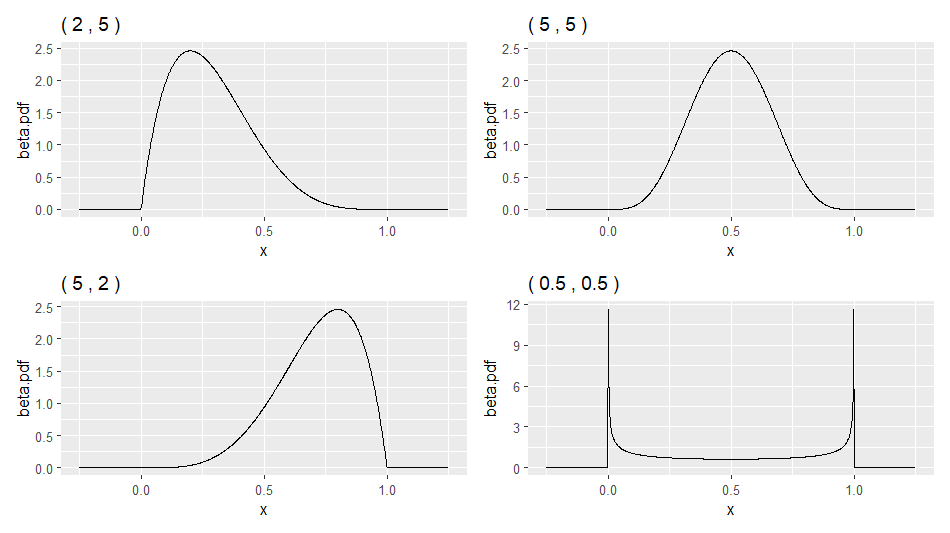
\includegraphics[width=\textwidth]{BetaDistributions.png}
    \caption{Beta dstribution for various $\alpha$ and $\beta$}
    \label{fig1}
   \end{minipage}
   \end{center}
\end{figure}

\begin{figure}[h]
  \begin{center}
  \begin{minipage}{0.75\textwidth}
    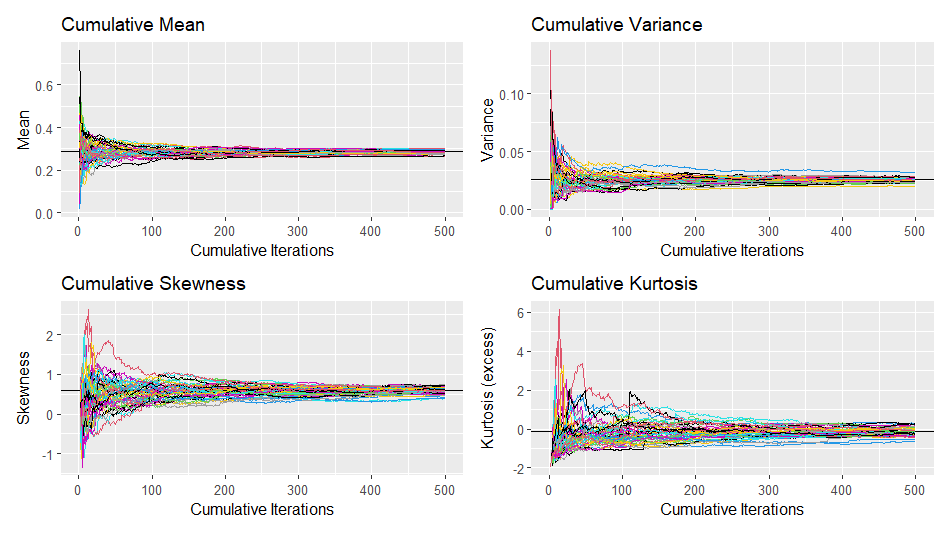
\includegraphics[width=\textwidth]{cumplots.png}
    \caption{Cumulative statistics up to sample size $n = 500$}
    \label{fig2}
   \end{minipage}
   \end{center}
\end{figure}

\begin{figure}[h]
  \begin{center}
  \begin{minipage}{0.50\textwidth}
    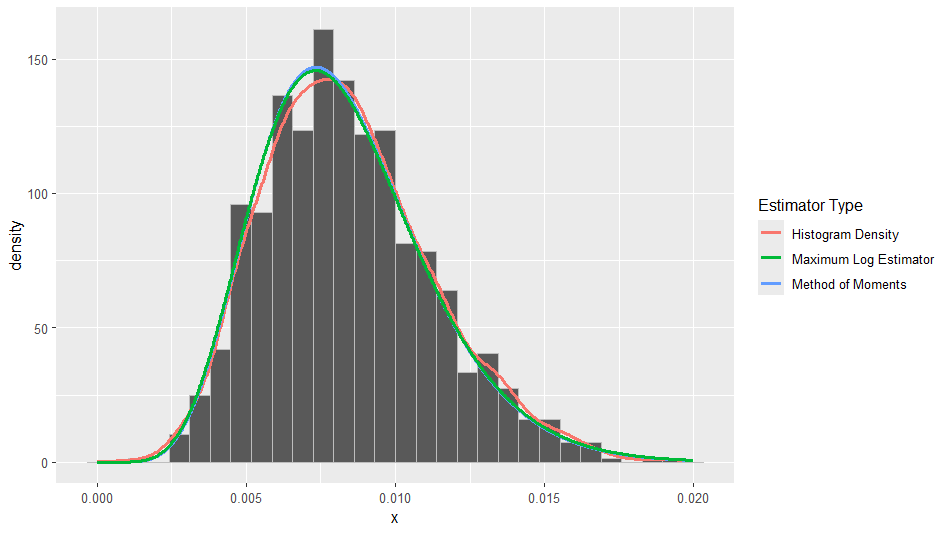
\includegraphics[width=\textwidth]{DeathRateBeta.png}
    \caption{Spread of death rates in 2022 modeled by histogram and beta distribution Approximations}
    \label{fig3}
   \end{minipage}
   \end{center}
\end{figure}

\begin{figure}[h]
  \begin{center}
  \begin{minipage}{0.50\textwidth}
    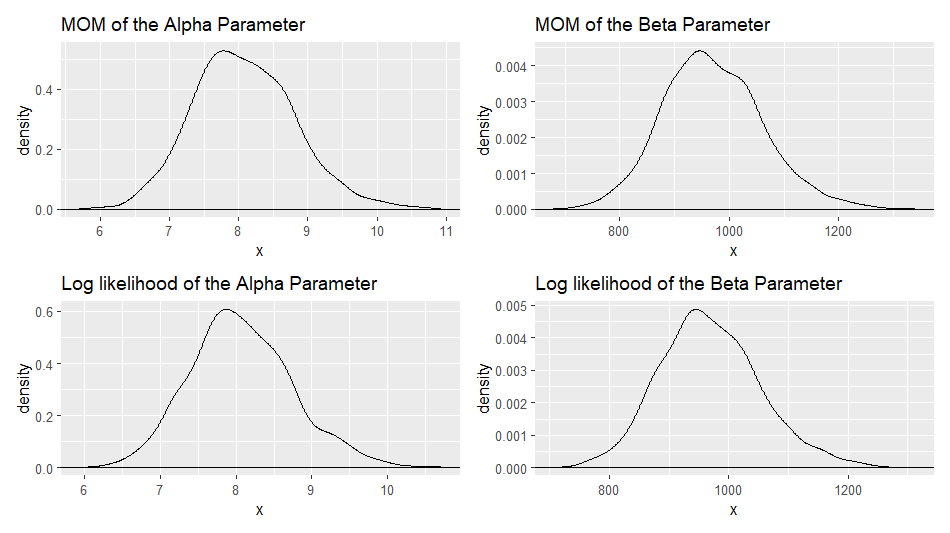
\includegraphics[width=\textwidth]{Parameters1000.png}
    \caption{Distributions of $n = 1000$ $\alpha$ and $\beta$ approximations for each point estimation method}
    \label{fig4}
   \end{minipage}
   \end{center}
\end{figure}

\begin{table}[h]
    \centering
    \begin{tabular}{|l|c|c|c|c|c|}
        \hline
        \textbf{Type} & \textbf{Distribution} & \textbf{Mean} & \textbf{Variance} & \textbf{Skewness} & \textbf{Kurtosis} \\
        \hline
        Population level & (2, 5)   & 0.2857  & 0.0255  & 0.5963  & -0.1200 \\
        Population level & (5, 5)   & 0.5000  & 0.0227  & 0.0000  & -0.4615 \\
        Population level & (5, 2)   & 0.7143  & 0.0255  & -0.5963 & -0.1200 \\
        Population level & (0.5, 0.5) & 0.5000  & 0.1250  & 0.0000  & -1.5000 \\
        \hline
        Integrated       & (2, 5)   & 0.2857  & 0.0574  & 2.4832  & 2.9565 \\
        Integrated       & (5, 5)   & 0.5000  & 0.0743  & 3.0999  & 2.4832 \\
        Integrated       & (5, 2)   & 0.7143  & 0.0574  & 3.3698  & 3.5982 \\
        Integrated       & (0.5, 0.5) & 0.5000  & 0.1406  & 1.4538  & 0.2652 \\
        \hline
        Sampled         & (2, 5)   & 0.2909  & 0.0271  & 0.5696  & 2.7784 \\
        Sampled         & (5, 5)   & 0.4976  & 0.0211  & 0.0645  & 2.5419 \\
        Sampled         & (5, 2)   & 0.7132  & 0.0262  & -0.7405 & 3.2192 \\
        Sampled         & (0.5, 0.5) & 0.5167  & 0.1199  & -0.1073 & 1.5461 \\
        \hline
    \end{tabular}
    \caption{Population level, integrated (MOM), and sampled distributions calculations}
    \label{tab1}
\end{table}

\begin{table}[h]
    \centering
    \begin{tabular}{|l|c|c|c|}
        \hline
        \textbf{Type} & \textbf{Bias} & \textbf{Precision} & \textbf{MSE} \\
        Alpha, MOM  & 0.0811  & 1.8286    & 0.5535 \\
        Beta, MOM   & 20.3346 & 0.0001    & 8768.2319 \\
        Alpha, Log  & 20.3346 & 2.7455    & 0.4752 \\
        Beta, Log   & 19.1844 & 0.0001    & 7566.8776 \\
        \hline
    \end{tabular}
    \caption{Bias, precision, and MSE for MOM and log likelihood}
    \label{tab2}
\end{table}


\end{document}
